

\chapter{Introduction}

\section{Getting Files from Subversion (svn) Repository}

The EPPIC files (and a history of all their changes) are stored in a
repository on the BU SCV machines. To  
access the files from one of the SCV machines, the command is

\begin{lstlisting}[language=BASH]
  # SOME COMMENTED NOTES:
  # svn = subversion program
  # co = short for checkout
  # file:///project/eregion/.astrosvn/eppic/trunk = the location of
  #      the repository and the paritcular subdirectory eppic/trunk  
  # eppic-svn = your local, linked copy of eppic will be stored in
  #      this directory 
  # 
  # THE COMMAND:
  svn co file:///project/eregion/.astrosvn/eppic/trunk eppic-svn
\end{lstlisting}

You may download the files from any other computer using your Kerberos
(login) account by using the following command:

\begin{lstlisting}[language=BASH]
  svn co svn+ssh://katana.bu.edu/project/eregion/.astrosvn/eppic/trunk eppic-svn
\end{lstlisting}

Checkout (co) is likely the only command in which you will need to
type/use the full path to the repository. Once \textbf{eppic-svn} is
created and you are working with it or it's subdirectories, svn will
know where the repository is by consulting hidden files. The two
exceptions are the svn commands 
\textbf{list} and \textbf{merge}. The first is useful to make sure you
are checking out the right directory by listing what files would be
downloaded if a checkout were performed. The second is a more involved
command that deals with managing several \emph{branches} of code. This
is a more advanced process to be discussed later on in seperate
chapter. 

In the next section, we briefly describe how to handle the build
system and compile the program for the first time. In a later chapter,
the details are laid out, but they are not important for understanding
the most important and common tasks to EPPIC development. The
following sections will cover more details of interacting with the
repository using Subversion.

\section{Special Compiling Instructrions}

When you download the EPPIC files you get along with the source code
a \textbf{configure} shell script and several \textbf{Makefile.in}
files, one for each directory. When run, \textbf{configure} turns the
\textbf{Makefile.in} files into Makefiles. These files can be used
with the \textbf{make} program to compile EPPIC. So the typical
installation process is:

\begin{lstlisting}[language=BASH]
cd eppic-svn
./configure
make 
make check
\end{lstlisting}

The last command runs a make \emph{target} that compiles and runs
several test programs, and this command is optional. This is the
typical install/compilation process, as is described in the user
manual. Sometimes during the development, the files involved in making
the \textbf{configure} and \textbf{Makefile.in} files need to be
changed, and these files will need to be recreated. This involves
several programs related to the GNU Autotools suite, including
\emph{autoconf, automake, autoheader,} and \emph{aclocal}. Since it's
pretty annoying to run all of these programs for minor changes, which
may be made frequently, on script was developed to call all of these
programs in the correct order: \emph{autoreconf}, so the compilation
process may involve the following process: 

\begin{lstlisting}[language=BASH]
cd eppic-svn
# --install tells autoreconf to add missing files
autoreconf --install
./configure
make 
make check
\end{lstlisting}

\subsection{Typical Development Session (using Subversion)}

... to come soon


%% * Version control and Repository
%% ** Intro
%%    SVN is used to keep a history of changes and to share revisions. It is just
%%    one of many [[http://betterexplained.com/articles/a-visual-guide-to-version-control/][version control]] systems out there, and there are many 
%%    [[http://msdn.microsoft.com/en-us/library/bb668955.aspx][stratagies]] for using them. You can access it using the command line, and
%%    there are online [[http://svnbook.red-bean.com/en/1.5/index.html][manuals]] to guide you in doing so (svn help /command/, works
%%    too). Finally, there is an emacs mode, [[http://www.xsteve.at/prg/emacs/psvn.el][psvn.el]], that can make life a lot
%%    easier (once this file is [[atbu_psvn][loaded]], you can activate this mode by pressing
%%    M-x and typing 'svn-status', followed by the directory you are using to hold
%%    your local copy of the eppic files).

%%    The main concecpt is to have a history of changes saved in a directory called
%%    a repository. Using SVN, you interact with this repository, 'downloading' and
%%    'uploading' changes and comments. You can download an old copy of the files
%%    or the latest. Your downloaded copy has an extra directory '.svn' in every
%%    directory of the local copy. This just helps SVN know where to find the 
%%    repository and what files should be copied over. DONT delete or move these 
%%    '.svn' directories, or things will get very confusing. 

%% ** Major Commands
%%    - 'svn checkout': get a fresh copy of the repository
%%    specifically,  'svn checkout
%%    svn+ssh://twister.bu.edu/project/nonadmd/.astrosvn/eppic/trunk eppic_dev'
%%    will get a copy form off-site.
%%    - 'svn update': while in your local copy, make sure the files are as new
%%      as possible
%%    - 'svn commit': submit your changes; -m message will record a message, but
%%      if you don't use this, the default text editor will open to ask for one. 
%%    - 'svn add /file/': this adds the file to the repository; WARNING: it wont
%%      actually be added until the following 'commit'.
%%    - 'svn add /directory/': add the directory and ALL the files in it.
%%    - 'svn mv': move a file in your copy and (after a commit) in the repository.
%%    - 'svn mkdir': make a new directory here and in the repository.

%% ** Conflicts
%%    Sometimes two people edit the same file,
%%    at the same time, 'uploading' one after another. The last person to submit 
%%    their changes has a conflict; in other words, their changes are temporarorly 
%%    rejected. The file is returned in a format similar to a 'diff' execution. 
%%    Sections that differ from one person's work to another's are placed back to
%%    back and highlighted with '<<<<<' and '====' lines. The person with the 
%%    conflict must decide which block to keep or how to mix the two. Three other
%%    files are returned when a conflict happens, all with the same name as the 
%%    rejected file but with different suffixes: .mine, .r**, r!!. ** and !! 
%%    will be two different numbers. ** will be how the file looked before either 
%%    person made changes. !! will be how the other person saved their work 
%%    (and changes). .mine will obviously be the way you have changed the file, 
%%    without all the '<<<<' and '====' sections. These are there to help in case
%%    the formating in the rejected file is confusing. Once all your work is done,
%%    'svn resolved' tells your .svn folder you are ready to actually save your 
%%    changes. Now commiting should happen cleanly

%% ** Update and Status
%%    'svn update' lists all the files in your local copy, each one preceeded by 
%%    a character. The characters have the following meanings:
%%    - ?: File is unknown to the repository; if it needs to be know, add it, but
%%      in many cases these are temporary files (*.o etc)
%%    - M: Modified file
%%    - C: Conflict
%%    - G: Confilct, but a simple diff ment an automatic resolution, ie two people
%%      edited the same file in distinctly different sections. 

%%    'svn status -u' reports the same information, but actually does nothing;
%%    this is useful incase you expect a conflict and you want to see where it 
%%    might happen.
   

%% ** A typical day using SVN

%%    1. Run 'svn update' or 'svn status -u' then 'svn update'
      
%%       If everyone is as current as possible, this will help limit conflicts.
%%    3. Make your changes. Hopefully these are small and take a few hours (or up 
%%       to a day or two) to complete. 
%%    4. Run 'svn update' or 'svn status -u' then 'svn update'
%%    5. Resolve any conflicts. 
%%    6. Run 'svn commit'
      
%%    We should be getting emails everytime someone makes changes, so there should
%%    be few suprises when an update is done.

\subsection{Preparing to Make Major Changes}

% describe how to start out on the process of a major change.

\subsection{Merging Major Changes WITHOUT Branches}

If you've been working on a local copy of the code but haven't updated
in a long time, this is the section for you. When you do run 
\begin{lstlisting}[language=BASH]
  svn update
\end{lstlisting}
\noindent you will see a list of files being changed in your local
copy. Next to each file, a single letter code will tell you how they
are being changed. Table \ref{t:svn_update_codes} describes these
codes.
\begin{table}\label{t:svn_update_codes}

\caption{Single letter codes SVN uses to describe the changes occuring
  during an update.}
\end{table}
\noindent The list will stop when you come to a conflict and you will
see a message like:
\begin{verbatim}
Conflict discovered in 'src/efield_quasineut.cc'.
Select: (p) postpone, (df) diff-full, (e) edit,
        (h) help for more options: 
\end{verbatim}
\noindent SVN will wait for your reply. The best option is 'p', which
says to move on with the update and create files used to deal with the
conflict:
\begin{lstlisting}[language=BASH]
  katana:~/eregion/eppic-r100 % svn update
.
.
.
U    src/main.cc
U    src/eppic-mpi.h
Conflict discovered in 'src/efield_quasineut.cc'.
Select: (p) postpone, (df) diff-full, (e) edit,
        (h) help for more options: p
C    src/efield_quasineut.cc
U    src/vpush_bc1.cc
A    src/rejectArrayNd.cc
.
.
.
\end{lstlisting}
\noindent This option creates three new files
(efield\_quasineut.cc.r100, efield\_quasineut.cc.r104, and
efield\_quasineut.cc.mine in this example) and modifies the
conflicting file (efield\_quasineut.cc). The suffix of the new files
tells you their source: .r100 is from the version prior to your
medeling, 100; .r104 is from the most current version (104) in the
repository, the one you are updating from; and .mine is just a copy of
your copy of efield\_quasineut.cc prior to the
update. efield\_quasineut.cc is also changed. It now has diff like
syntax at each conflicting location, to make it easy to identify
differences and make changes. Just search for the blocks beginning
with the line '<<<<<<< .mine'. From this line to the '======='
line, is your work. Then onto the line looking like '>>>>>>> .r104' is
what is now in the repository. The tough part is decide how to resolve
the differences. 
 
\subsection{Merging Major Changes Using Branches}


   Sometimes your edits will take more than a day to complete. For this we use
   what are called branches. A branch is just an efficient duplication of the
   repository, in the repository. In other words it's like having two
   repositories, whose  
   histories will deviate a bit. Once all the work is done,
   \begin{lstlisting}[language=BASH]
     svn merge /repo1/ /repo2/ /result_dir/
   \end{lstlisting}
   \noindent is used to do the equivilant of a
   commit from repo1 to repo2, but it saves all the files, conflicts or not,
   in the /result\_dir/. Once all the conflicts are resolved, they are saved in
   one of the branches, and the other is left alone.

   How is this typically used? There is a repository directory called 'trunk',
   and it contains the copy of the files (and history) of the main program. 
   Any major modification get's it's own copy, in it's own folder, for example
   'inject\_dev'. The 'trunk' copy of the code will be updated for bugs and 
   minor improvements. The 'inject\_dev' will involve major changes. While
   these changes are done, bug fixes from the main 'trunk' are periodicly 
   integrated by the 'inject\_dev' developer by performing 
   'svn merge /trunk/ /inject\_dev/ /myinject\_dev\_wbugfix/'. After each of these,
   work continues in the /myinject\_dev\_wbugfix/ local copy. At the end of all 
   this, there will be a final merge, which should be minor because of the 
   periodic merges, and the results are commited back to the 'trunk'. Since it
   has served it's purpose, the 'inject\_dev' branch is ignored from then on.

   Branches are also used as markers. We will make branches called 'version1',
   'version2',... etc., and because these branches are efficient copies, they
   don't take up much space. It makes it easy though to grab the latest 'stable'
   verstion, since you can checkout one branch over another (forexample the 
   main development trunk). 

\section{Using Branches as Milestones, or the Branch Strategy}
%% ** Branch Stategy

%% #+BEGIN_LaTeX
%%    \begin{center}
%%    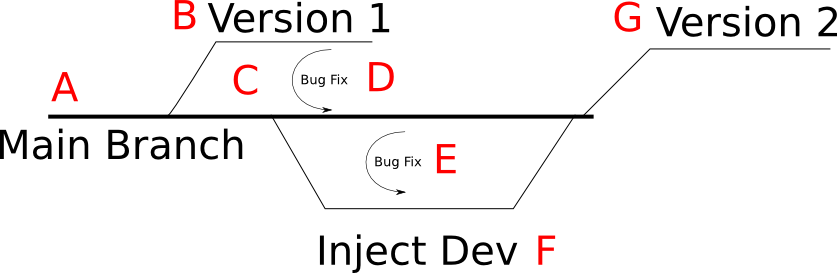
\includegraphics[width=.8\textwidth]{/usr3/graduate/yannpaul/eregion2/eppic_dev/doc/svn_how_to.png}
%%    \end{center}
%% #+END_LaTeX   
%% #+BEGIN_HTML
%%    <img src="svn_how_to.png"/>
%% #+END_HTML
%%    A. The repository has a branch called 'trunk', where the general history is
%%       kept.

%%    B. At some point, we decide to isolate 'version 1', because X amount of 
%%       features work and are (mostly) reliable. 

%%    C. A major change is needed, so we make a seperate branch: 'inject dev'

%%    D. A bug is found in version 1, fixed and it's change is merged with the 
%%       'trunk'

%%    E. The bug fix is passed along to 'inject dev' from the 'trunk' through a 
%%       merge. 

%%    F. Work on 'inject dev' is done, and it is merged with the 'trunk'.

%%    G. Now that new features are added, 'version 2' is created. 

%%    Point (C) can be eliminated if 'version 1' is really expected to be 
%%    only used as a marker. Some programs have their most recent 'stable' version
%%    updated only for bug fixes, as soon as they are found and fixed, while
%%    others don't touch a 'stable' version and bug fixes are made to the trunk.
%%    In this second case, the fixes are shared with the users after only another
%%    stable version is released. 
   


